\section{Telemetry Module}

The telemetry module implements the design specified in Sec.\ \ref{sec:Telemetry-Module-Design}. The hardware and software aspects of this module's implementation are discussed in this section. Figure \ref{fig:telemetry_pcb} shows a photo of the completely populated and debugged telemetry module hardware.

\begin{figure}[H]
\centering
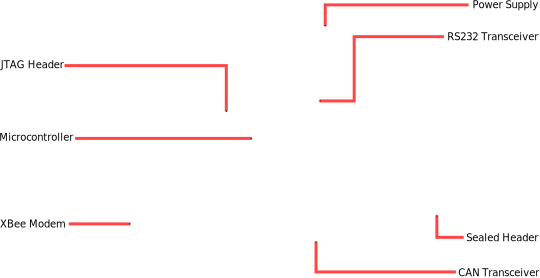
\includegraphics[scale=1]{implementation/figures/telemetry_pcb.eps}
\caption{Photograph of the populated telemetry module PCB.}
\label{fig:telemetry_pcb}
\end{figure}

\subsection{Hardware}

In addition to the base system hardware common to all modules described in Sec.\ \ref{sec:base_system_hardware}, several additional components were required in the implementation of the telemetry module. A block diagram of the telemetry module hardware implementation is shown in Fig.\ \ref{fig:telemetry_hardware_block}. The additional components are summarized in in Table \ref{tab:telemetry_module_components}.

\begin{figure}[H]
\centering
\def\antenna{
  -- +(0mm,4.0mm) -- +(2.625mm,7.5mm) -- +(-2.625mm,7.5mm) -- +(0mm,4.0mm)
}

\begin{tikzpicture}[auto, node distance=4cm, draw=black!70, >=stealth']
  \node [block, name=max3100] {Max3100 SPI UART};
  \node [block, name=at90, right of=max3100] {AT90CAN};
  \node [block, name=rs232, right of=at90] {Max232 RS232 Transceiver};
  
  \node [block, name=can, below of=at90, above=1cm] {MCP2551 CAN Transceiver};
  \node [block, name=modem, left of=can] {XBee Modem};
  
  \node [block, name=ecu, right of=rs232] {ECU};
  \node [block, name=dac, below of=ecu, above=1cm] {DAC};

  \path (at90.north)+(0.0,+0.4) node (title) {Telemetry Module};

   \begin{pgfonlayer}{background}
       \path (max3100.north west)+(-0.3,0.7) node (a) {};
       \path (can.south -| rs232.east)+(+0.3,-0.2) node (b) {};
       \path[module] (a) rectangle (b);
   \end{pgfonlayer}

  \node [bus, name=can1, below of=can, label=below:CAN Bus, above=2.5cm] {CAN Bus};
  \node [bus, name=can2, left of=can1] {};
  \node [bus, name=can3, right of=can1] {};

  \draw [-, thick] (modem.west) -| ($(modem.west)+(-0.8,0.2)$) \antenna;

  \draw [-, line width=3pt] (can) -- (can1);
  \draw [-, line width=3pt] (can1) -- (can2);
  \draw [-, line width=3pt] (can1) -- (can3);

  \draw [<->, thick] (at90) -- node[] {SPI} (max3100);
  \draw [<->, thick] (max3100) -- node[text width=2cm] {Serial} (modem);
  \draw [<->, thick] ($(at90.east)+(0,0.1)$) to[myncbar, arm=1cm] ($(rs232.north west)+(0,-0.5)$);
  \draw [<-, thick] ($(at90.east)+(0,-0.1)$) to[myncbar, arm=1cm] ($(rs232.south west)+(0,+0.5)$);

  \draw [<->, thick] ($(rs232.north east)+(0,-0.5)$) to[myncbar, arm=1cm] (ecu);
  \draw [<-, thick] ($(rs232.south east)+(0,0.5)$) to[myncbar, arm=1cm] (dac);

  \draw [<->, thick] (at90) -- (can);

%  \draw [<->, thick] (modem) -- node[] {} (telemetry);
%  \draw [<->, thick] (telemetry) -- node[] {RS232} (ecu);
%  \draw [<->, thick] (telemetry) -- node[] {RS232} (daq);
%  \draw [-, thick] (modem) -- node[text width=1.5cm] {} (ant) \antenna;
\end{tikzpicture}
\caption{Overview of the telemetry module hardware.\label{fig:telemetry_hardware_block}}
\end{figure}

\begin{table}[H]
  \caption{List of components used by the telemetry module.}
  \centering
    \begin{tabular}{|c|c|c|}
      \hline 
      Part & Manufacturer & Part Number\tabularnewline
      \hline
      \hline
      XBee-PRO OEM Module & Digi International & XBee-PRO\tabularnewline
      \hline 
      Dual RS-232 Transceiver & Maxim Electronics & MAX232\tabularnewline
      \hline 
      SPI-capable UART chip & Maxim Electronics & MAX3100\tabularnewline
      \hline 
      300mA Low Dropout Regulator & Linear Technology & LT1521\tabularnewline
      \hline
      8-bit dual-supply level translator & ST Microelectronics & ST2378E\tabularnewline
      \hline
    \end{tabular}
    \label{tab:telemetry_module_components}
\end{table}

\subsubsection{MAX232 Dual RS-232 Transceiver}

The ECU and the DAQ modules connect to the telemetry board with specialized cables that connect to the wiring harness. The ECU and DAQ interface with two built-in USART ports on the AT90CAN128 micro-controller. A Maxim brand MAX232 dual RS-232 transceiver chip is used to interface the built-in USARTs with the serial ports on the ECU and DAQ.

\subsubsection{XBee-PRO Wireless Modem}

To meet the range and data throughput requirements for the telemetry system, an XBee-PRO wireless modem is used. The XBee requires a \unit{3.3}{\volt} supply and logic levels, so the LT1521 \unit{3.3}{\volt} linear voltage regulator from Linear Technology is used to power the XBee-PRO. A separate antenna port is connected to the modem and mounted in the side of the module enclosure.

\subsubsection{MAX3100 SPI-based UART}
\nomenclature{IRQ}{Interrupt Request}

Since the AT90CAN129 has only 2 built-in UARTS that are used for the RS-232 interfaces to the ECU and DAQ, a third external UART is used to communicate with the XBee-PRO. The Maxim brand MAX3100 is an SPI-interfaced UART with an 8 word deep FIFO buffer. It features an active-low \emph{interrupt request} (IRQ) line connected to an external interrupt on the micro-controller. This external hardware interrupt line is used to signal the micro-controller whenever new data arrives or has been successfully sent.

\subsubsection{ST2378E 8-Bit Level Translator}

Since the XBee-PRO, MAX3100, and AT90CAN128 all operate at different logic levels, a dual-supply level translator is required. The ST Microelectronics' ST2378E is an ideal choice, as it can handle the high-frequency signal transitions that occur during data transmission. Signals between the XBee PRO, MAX3100, and the ST2378E use \unit{+3.3}{\volt} logic, while signals between the AT90CAN128 and the high-supply side of the ST2378E use \unit{+5}{\volt} logic.

\subsection{Software}

The module software is concerned primarily with transferring data to and from the ECU, DAC, and their respective remote software applications with as much data throughput as possible. An overview of the telemetry module's system software can be seen in Fig.\ \ref{fig:telemetry_software_implementation}. As is common with all our implementations, a hardware abstraction layer provides an easy-to-use interface to the hardware for the module software.

\begin{figure}[H]
\centering
\begin{tikzpicture}[auto, node distance=2cm, draw=black!70, >=stealth']
%  \draw[help lines] (-3,-5) grid (8,2);
  
  % Usart0 section
  \node [blue shiny, rectangle, minimum width=2cm] (usart0) {UART0};
  \node [blue shiny, rectangle, above of=usart0, node distance=1cm] (ecu) {ECU};

  \node [red shiny, rectangle, below of=usart0, right=-1cm, node distance=1cm] (usart0_rx) {Rx};
  \node [red shiny, rectangle, below of=usart0, left=-1cm, node distance=1cm] (usart0_tx) {Tx};

  \draw [<->] (ecu) to (usart0);
  \draw [<-] (usart0_rx) -- ($(usart0.south west)!(usart0_rx.north)!(usart0.south east)$);
  \draw [->] (usart0_tx) -- ($(usart0.south west)!(usart0_tx.north)!(usart0.south east)$);
  
  % Max3100 section
  \node [blue shiny, rectangle, minimum width=2cm, right of=usart0, node distance=3cm] (max3100) {MAX3100};
  \node [blue shiny, rectangle, above of=max3100, node distance=1cm] (xbee) {Xbee};
  \node [blue shiny, rectangle, below of=max3100, above=-0.3cm, left=0.25cm, node distance=0, font=\tiny, inner sep=0.075cm] (max3100_rx_hw) {Rx};

  \node [red shiny, rectangle, below of=max3100, right=-1cm, node distance=1cm] (max3100_rx) {Rx};
  \node [red shiny, rectangle, below of=max3100, left=-1cm, node distance=1cm] (max3100_tx) {Tx};

  \draw [<->] (xbee) to (max3100);
  \draw [<-] (max3100_rx) -- ($(max3100_rx_hw.south west)!(max3100_rx.north)!(max3100_rx_hw.south east)$);
  \draw [->] (max3100_tx) -- ($(max3100.south west)!(max3100_tx.north)!(max3100.south east)$);

  \node [red shiny, rectangle split, rectangle split parts=3, below of=max3100, text width=1.8cm, font=\scriptsize, text centered,
	  minimum width=2cm, anchor=base] (xbee_library)
    {XBee Library
      \nodepart{second} Packetizer
      \nodepart{third} Packet Buffer};

  %\node [red shiny, rectangle, below of=packetizer, node distance=1cm, minimum width=2cm,
%	  text width=1.75cm, font=\scriptsize, text centered] (packet_buf) {Rx Packet Buffer};

  \draw [->] (max3100_rx) -- ($(xbee_library.north west)!(max3100_rx.south)!(xbee_library.north east)$);
  \draw [<-] (max3100_tx) -- ($(xbee_library.north west)!(max3100_tx.south)!(xbee_library.north east)$);

  % Usart1 section
  \node [blue shiny, rectangle, minimum width=2cm, right of=max3100, node distance=3cm] (usart1) {UART1};
  \node [blue shiny, rectangle, above of=usart1, node distance=1cm] (dac) {DAC};

  \node [red shiny, rectangle, below of=usart1, right=-1cm, node distance=1cm] (usart1_rx) {Rx};
  \node [red shiny, rectangle, below of=usart1, left=-1cm, node distance=1cm, dashed] (usart1_tx) {Tx};

  \draw [<->] (dac) to (usart1);
  \draw [<-] (usart1_rx) -- ($(usart1.south west)!(usart1_rx.north)!(usart1.south east)$);
  \draw [->, dashed] (usart1_tx) -- ($(usart1.south west)!(usart1_tx.north)!(usart1.south east)$);

  \node [red shiny, rectangle split, rectangle split parts=4, below of=usart1, text centered, minimum width=2cm, anchor=base, text width=1.85cm, inner xsep=0, font=\scriptsize] (dac_library)
    {DAC Library
      \nodepart{second} Buffer
      \nodepart{third} Decoder
      \nodepart{fourth} Encoder};

  \draw [->] (usart1_rx) -- ($(dac_library.north west)!(usart1_rx.south)!(dac_library.north east)$);
  \draw [<-, dashed] (usart1_tx) -- ($(dac_library.north west)!(usart1_tx.south)!(dac_library.north east)$);

  % CAN stuff
  \node [blue shiny, rectangle, minimum width=2cm, right of=usart1, node distance=3cm] (can) {CAN};
  \node [red shiny, rectangle, minimum width=2cm, below of=can, node distance=1cm] (can_driver) {Driver};

  \node at (dac_library.third split -| can_driver)
	    [red shiny, rectangle, minimum width=2cm, text width=1.85cm, font=\scriptsize, text centered] (can_library) {Telemetry CAN Library};

  \draw [<->] (can) -- (can_driver);
  \draw [<->] (can_driver) -- (can_library);

  \draw [->] (dac_library.third east) -- ($(can_library.north west)!(dac_library.third east)!(can_library.south west)$);
  \draw [<-] (dac_library.fourth east) -- ($(can_library.north west)!(dac_library.fourth east)!(can_library.south west)$);

  % Now for the rest of the connections
  \draw [->] (xbee_library.third west) -| (usart0_tx);
  \draw [<-] (xbee_library.second west) -| (usart0_rx);
  \draw [->] (dac_library.second west) to node [name=mid1] {} (xbee_library.second east);
  \draw [->] (dac_library.fourth west) -| (mid1);

  \node [left of=usart0, node distance=3cm, minimum width=3.5cm] (perifs) {Module Periferals};
  \node [below of=perifs, node distance=1cm, minimum width=3.5cm] (buffers) {Drivers/Buffers};
  \node [below of=buffers, node distance=1cm, minimum width=3.5cm] (libraries) {Libraries};

  \begin{pgfonlayer}{background}
    \path (perifs.north west)+(-0.0,0.1) node (a1) {};
    \path (can.south east)+(+0.1,-0.1) node (b1) {};
    \path[draw=blue!50!black!50, rounded corners=0.1cm] (a1) rectangle (b1);

    \path (buffers.north west)+(-0.0,0.1) node (a2) {};
    \path (can_driver.south east)+(0.1,-0.1) node (b2) {};
    \path [draw=red!50!black!50, rounded corners=0.1cm] (a2) rectangle (b2);

    \path (libraries.north west)+(-0.0,0.1) node (a3) {};
    \path (can_library.south east)+(0.1,-0.1) node (b3) {};
    \path [draw=red!50!black!50, rounded corners=0.1cm] (a3) rectangle (b3);
  \end{pgfonlayer}

  % Guide
  \node at ($(a3 |- b3)+(0.0,-0.1)$) [anchor=north west, blue shiny, minimum width=2cm] (hardware) {Hardware};
  \node [red shiny, right of=hardware, node distance=2.2cm, minimum width=2cm] (software) {Software};
  
\end{tikzpicture}

\caption{Overview of the telemetry module software.}
\label{fig:telemetry_software_implementation}
\end{figure}

\subsubsection{MAX3100 UART Driver}

The software driver written for the MAX3100 shares it's interface and buffer code with the built-in AT90CAN128 USART driver described in Sec. \ref{sec:impl_spi_driver}. The statically-allocated circular buffer approach first introduced with the built-in USART is left unchanged. 

The MAX3100 provides asynchronous transmission and reception of data with an external hardware interrupt signal. A flow-chart of the hardware interrupt service routine is shown in Fig.\ \ref{fig:usart_driver_flow}. The MAX3100 driver allows the module software to define callback functions to be executed when new data arrives or has been transmitted. 

\begin{figure}[H]
\centering
\begin{tikzpicture}[auto, node distance=2cm, draw=black!70, >=stealth']
  \node [start] (int) {Interrupt};
  \node [decision, right of=int, right=0cm] (rx) {Rx Byte?};
  \node [block, below of=rx] (add) {Add to Rx buf.};

  \node [decision, right of=rx, right=0cm] (tx) {Tx Byte?};
  \node [block, below of=tx, text width=2.5cm, inner xsep=0pt] (remove) {Remove from Tx buf.};
  \node [end, right of=tx, right=0cm] (return) {Return};

  \draw [->] (int) -- (rx);
  \draw [->] (rx) to node [] {yes} (add);

  \draw [->] (rx) -- node [name=mid] {no} (tx);
  \draw [->] (add) -| (mid);

  \draw [->] (tx) to node [] {yes} (remove);
  \draw [->] (tx) -- node [name=mid2] {no} (return);
  \draw [->] (remove) -| (mid2);

\end{tikzpicture}
\caption{Flow-chart of the USART interrupt service routine.}
\label{fig:usart_driver_flow}
\end{figure}

The MAX3100 driver is configured to use a $\unit{4}{\mega\hertz}$ SPI clock to meet the data throughput requirements demanded from multiplexing the DAC and ECU streams. It interfaces directly with the SPI driver described in Sec. \ref{sec:impl_spi_driver}.

\subsubsection{XBee PRO Library}

To route data to and from the ECU, DAC, and laptop, the module software must utilize the special ``API'' mode described in the XBee documentation \cite{XBeeManual}. The API mode allows the packetizing of data required to multiplex two serial streams onto one transmission channel. The XBee PRO library implements two critical functions:

\begin{enumerate}
\item To send and receive packetized data to and from the user software ; and
\item To switch the modem into API mode, and manage the modem's settings.
\end{enumerate}

The XBee library contains two major functions: one to packetize outgoing data for the main control loop software, and one to disassemble incoming packets and provide their payload to the main control loop.

The XBee library implements a binary packet protocol described in the XBee manual, and is able to send and receive unicast and multicast packets to addressable end-points. Each end-point corresponds to a virtual serial port on the receiving laptop. The modem supports full 64-bit addresses, but the driver only implements a 16-bit addressing mode as the extra address space is not required. The driver is also capable of sending commands to the modem and interpreting it's response.

The module software can send a packet by supplying the driver with the target address, a pointer to the data, and the number of bytes. The driver automatically constructs the XBee packet and buffers the data for transmission. Receiving packets is more complicated, since individual bytes arrive at the MAX3100 drivers's RX buffer asynchronously. A receiver state machine waits for a full packet to be available in the RX buffer, and then pushes it into a separate incoming packet buffer. This incoming packet buffer can then be read by the module software.

Since minimal configuration functionality is required, only a handful of modem commands are implemented. The driver is able to place the modem into API mode, after which all communication is done using the packet interface. The modem commands implemented by the telemetry Module are listed in Table \ref{tab:xbee_commands}.

\begin{table}
\caption{List of implemented XBee modem commands.}
\centering{}
\begin{tabular}{|l|l|}
\hline 
Command & Description \tabularnewline
\hline
\hline
AP & Set and read the API mode state. \tabularnewline
\hline
CH & Set and read the RF channel. \tabularnewline
\hline 
ID & Set and read the PAN (Personal Area Network) ID. \tabularnewline
\hline
MY & Set and read the modems local address. \tabularnewline
\hline
\end{tabular}
\label{tab:xbee_commands}
\end{table}

The XBee modem can be controlled out of API mode by entering into it's command mode by sending a special string of bytes. A list of modem-style AT-commands, documented in the manual, are used to change the various settings of the modem. This command mode was used initially to set up the modems by hand, but is now only used by the software on startup to enable the API mode.

The XBee library makes use of the familiar ``callback'' concept to provide the user software with incoming data. Function pointers are used to connect the library to a UART, which makes it possible to reconfigure the library to use a different USART on-the-fly.

\subsubsection{DAC Library}
\label{sec:dac_library}

Special routines for decoding the DAC data stream and constructing new DAC data packets are required to meet the requirements described in Section \ref{sec:Telemetry-Module-Design}. These routines are packaged into a DAC library for use by the module software.

The DAC library maintains it's own buffer of incoming DAC data. Separate functions exist for buffering incoming data and for processing that data. The library uses the callback feature of the USART to pass incoming bytes to it's own buffer. Transmission of DAC data over the wireless link is synchronized with the DAC library decoder. Whenever an entire DAC packet is decoded by the library, that packet is then buffered for transmission by the modem.

\subsubsection{Main Control Loop}

Once the module hardware has been initialized and the XBee has successfully entered API mode, the telemetry module's enters it's main control loop. This loop performs three tasks:

\begin{enumerate}
  \item The ECU USART receive buffer is polled for data. If there is any incoming data waiting, send it over the ECU link by passing it to the packetizer;
  \item Any incoming packets in the XBee receive buffer are routed to the appropriate end-point, either the ECU USART or DAC driver; and
  \item The DAC decoder function checks to see if any the data in the DAC's incoming data buffer can be decoded into a valid DAC packet.
\end{enumerate}

The main control loop runs these three tasks over and over, processing incoming data as it arrives, and routing outgoing data as needed. 
